\documentclass[conference]{IEEEtran}
\usepackage{graphicx}
\usepackage{booktabs}
\usepackage{amsmath}
\usepackage{amssymb}
\usepackage{xcolor}
\usepackage[hidelinks]{hyperref}

\graphicspath{{figs/}}

\title{How Much Headroom Do Placement Schedules Have?\\
A Noise-Calibrated Study of LLM-Evolved Schedules\\
in Differentiable VLSI Placement}

% TODO: set your preferred author name/affiliation before submission
\author{\IEEEauthorblockN{Chaithu Talasila}
\IEEEauthorblockA{Independent Researcher\\
\texttt{github.com/themoddedcube/evoplace}}}

\begin{document}
\maketitle

\begin{abstract}
Large language models (LLMs) have recently been used to evolve algorithmic
components of GPU-accelerated analytical placers, with reported wirelength
improvements of 5--17\% on macro-heavy benchmarks. We investigate a
component class untouched by prior work: the smoothness ($\gamma$) schedule
of the weighted-average wirelength model in DREAMPlace. We present
EvoPlace\footnote{Our system was developed under this name prior to our
awareness of the concurrent, independent system of Yao et
al.~\cite{yao2025evolution} bearing the same name; we retain it for
repository consistency and cite their work explicitly throughout.}, an
evolution harness built on three components: (i)~a hook-injection layer
that lets a candidate schedule---a pure Python function---steer an
unmodified DREAMPlace build; (ii)~a cascade evaluator with stage-matched
baselines that rejects poor candidates at $13\times$ lower cost than a full
placement; and (iii)~a \emph{noise-calibrated evaluation protocol} that
measures the single-seed fitness noise floor ($\sigma\!\approx\!0.15\%$
normalized HPWL), gates every campaign on hook-liveness probes, and
confirms final rankings with paired multi-seed re-evaluation. Two complete campaigns
on ISPD~2015 standard-cell designs yield an instructive contrast. The
$\gamma$ (wirelength-smoothing) campaign produced exactly one
statistically real improvement over 200 iterations---$+0.315\%\pm0.09\%$
(SEM)---and its single-seed ranking \emph{inverted} under multi-seed
re-evaluation, bounding the $\gamma$-search headroom near $0.3\%$. The
$\lambda$ (density-weight) campaign found its result before evolution
began: constructing a default-matched seed exposed that DREAMPlace's
HPWL-feedback guard in the density-weight update \emph{actively hurts}
these designs---removing it wins $1$--$9\%$ HPWL at matched final density,
$14/14$ paired seeds across four designs, a generalizing improvement found
by \emph{audit}, not search. Evolution on top of the audited seed found
nothing: an unguarded HPWL fitness was reward-hacked within nine
iterations (candidates scored well by refusing to spread cells), and after
adding a density gate, zero of 200 candidates beat the seed. We conclude
that schedule \emph{search} offers noise-level headroom, while
\emph{auditing} the hand-tuned adaptive heuristics it competes against
does not---and that a noise-calibrated, gate-checked protocol is what
separates both findings from the artifacts an uncalibrated loop happily
reports.
\end{abstract}

\section{Introduction}

Analytical global placement casts cell spreading as continuous
optimization: DREAMPlace~\cite{lin2019dreamplace} expresses the ePlace
electrostatic formulation~\cite{lu2015eplace} in a deep-learning toolkit
and achieves order-of-magnitude speedups on GPUs. The objective combines a
smooth approximation of half-perimeter wirelength (HPWL) with an
electrostatic density penalty, minimized by Nesterov's method. Two scalar
\emph{schedules} steer this optimization: the weighted-average wirelength
smoothness parameter $\gamma$, which trades gradient smoothness against
HPWL fidelity, and the density weight $\lambda$. Both are hand-designed
heuristics, tuned by experts over years.

A natural question follows from the recent success of LLM-guided
algorithm evolution~\cite{novikov2025alphaevolve}: can an LLM discover a
better schedule? Concurrent work has evolved other DREAMPlace components
---initialization, preconditioner, and optimizer---reporting case-by-case
HPWL reductions of 5--8\% on average~\cite{yao2025evolution}. Schedules,
however, were not examined, and the reliability of small reported gains in
this field is clouded by a methodological hazard: placement is stochastic,
single-seed evaluation is near-universal, and few studies report variance
at all~\cite{cheng2023assessment,markov2023false}.

This paper reports a complete, noise-calibrated campaign of LLM-guided
$\gamma$-schedule evolution. Our contributions are:
\begin{itemize}
  \item \textbf{A measurement-first evolution harness.} Schedule
        candidates are pure Python functions injected into an unmodified
        DREAMPlace build through a hook layer; the evaluation harness is
        frozen for the life of the campaign; and a cascade evaluator with
        \emph{stage-matched baselines} rejects 93\% of candidates at a
        fraction of full-evaluation cost.
  \item \textbf{A noise-calibrated evaluation protocol.} We measure the
        single-seed fitness noise floor, gate the campaign on differential
        hook-liveness probes, and confirm all final claims by paired
        multi-seed re-evaluation against the default schedule on identical
        (benchmark, seed) pairs.
  \item \textbf{A quantitative boundary result for $\gamma$.} Across 200
        evolution iterations, the best schedule that survives multi-seed
        scrutiny improves HPWL by $0.315\%\pm0.09\%$; the single-seed
        winner is revealed as noise.
  \item \textbf{An audit finding larger than the search.} Removing the
        HPWL-feedback guard from DREAMPlace's density-weight update
        improves HPWL by $1$--$9\%$ at matched final density ($14/14$
        paired seeds, four designs) --- discovered through the protocol's
        own parity gate, not through evolution.
  \item \textbf{A live characterization of fitness under-specification.}
        With an HPWL-only fitness, $\lambda$-schedule evolution
        reward-hacks within nine iterations by suppressing cell spreading;
        with an explicit density gate, the same search finds nothing in
        200 iterations. Every metric a candidate can influence requires a
        gate.
\end{itemize}

We deliberately report a bounded-headroom (negative) result with full
provenance, including a record-keeping artifact we caught and corrected.
In a field where almost no small improvement is variance-qualified, we
believe the calibration methodology is as much a contribution as the
bound itself.

\section{Related Work}

\textbf{GPU-analytical placement.} DREAMPlace~\cite{lin2019dreamplace}
implements ePlace/RePlAce-style electrostatic placement with CUDA kernels
under a PyTorch-like API; successive versions added timing-driven net
weighting and mixed-size support. Its $\gamma$ schedule follows an
overflow-driven exponential heuristic; our seed program reproduces this
default to machine precision so that evolution starts from parity.

\textbf{LLM-evolved placement components.} Yao et
al.~\cite{yao2025evolution} evolve initialization, preconditioner, and
optimizer implementations with GPT-4o at scale ($\geq$1000 candidates per
component, $\sim$210 GPUs), reporting 5.05--8.30\% average case-by-case
HPWL reductions, with initialization dominating and an order-of-magnitude
collapse when one evolved algorithm must generalize across designs. Their
clean standard-cell-like cases improve by only 0.03--0.59\%---consistent
with the bound we measure for schedules. VeoPlace~\cite{veoplace2026}
evolves macro placements with vision-language-model feedback and is one of
the few systems in this space to report multi-seed means with standard
errors.

\textbf{Evaluation reliability in ML-for-EDA.} The reassessments of
RL-based macro placement~\cite{mirhoseini2021graph} by Cheng et
al.~\cite{cheng2023assessment} and Markov~\cite{markov2023false}
demonstrated that headline gains can be artifacts of undisclosed
initialization and weak baselines. RoutePlacer~\cite{routeplacer2024} is a
rare example reporting mean$\pm$std over five seeds. Our protocol extends
this thread: we \emph{measure} the noise floor first and require any
claimed improvement to clear it under paired re-evaluation.

\section{The EvoPlace Harness}
\label{sec:system}

\subsection{Hook injection}
A patched \texttt{PlaceObj} consults a module-level hook registry at every
global-placement iteration. When a candidate registers
\texttt{gamma\_schedule(iteration, total\_iterations, overflow,
hpwl\_history)}, its return value (clamped to a documented range)
overrides the built-in heuristic; when no hook is set, DREAMPlace behaves
identically to upstream. Candidates are therefore pure Python functions,
loaded dynamically---no rebuild, no source swap. The same registry exposes
$\lambda$-schedule, initialization, and timing-loss slots.

\subsection{Frozen evaluator and cascade}
A fixed harness (\texttt{evaluator/run\_placement.py}) builds DREAMPlace
parameters from per-benchmark JSON, injects hooks, runs placement to
convergence (stop overflow 0.07, legalization included), and extracts
final HPWL and overflow. The file is never modified during a campaign,
preventing fitness-definition drift. Candidate evaluation uses a
three-stage cascade (50, 300, 2000 iterations) with rejection thresholds
(2.0, 1.3) normalized against \emph{stage-matched} baselines: a truncated
run of the default schedule lands $2$--$2.5\times$ above its converged
HPWL, so normalizing truncated candidates against converged baselines
would cull everything, including the default itself. Stage-0 rejection
costs ${\sim}5$\,s versus ${\sim}30$\,s for a full pass on our hardware.

\subsection{Evolution loop}
We drive evolution with an OpenEvolve-style loop: MAP-Elites over
(normalized HPWL, convergence speed) with four islands of 25 programs,
diff-based mutations from a Claude model ensemble (temperature 0.8), and
TSV logging of every candidate with code hashes. A lightweight
hill-climbing fallback loop shares the same evaluator.

\section{Noise-Calibrated Evaluation Protocol}
\label{sec:protocol}

\textbf{Noise floor.} Repeated full placements of the \emph{same} schedule
under different seeds establish a single-seed fitness standard deviation
of $\sigma\approx0.15\%$ normalized HPWL on our benchmarks. Every
single-seed score in the campaign is interpreted against this floor; we
pre-registered the rule that no single-seed improvement below
$3\sigma\approx0.45\%$ may be treated as a result.

\textbf{Liveness gating.} An earlier CPU-era campaign of ours silently
evaluated \emph{vanilla DREAMPlace for every candidate}---the hooks were
not wired into the installed tree---producing 20 near-identical scores
whose spread was pure numerical noise. The failure motivated two standing
gates run before any campaign: (i)~the seed program must reproduce the
default baseline at $\text{norm.\ HPWL}=1.0\pm0.01$ through the real
cascade; and (ii)~a \emph{differential probe}---a deliberately degenerate
schedule (constant $\gamma=0.01$)---must produce a markedly different
outcome (in practice, cascade rejection). Together these prove the
candidate code path actually steers the placement.

\textbf{Paired multi-seed confirmation.} After a campaign, top candidates
and the seed program are re-evaluated with full placements on a grid of
(benchmark, seed) pairs; each run is normalized by the \emph{default
schedule's HPWL on the identical pair}. Pairing cancels per-seed placement
luck. The seed program rides along as a calibration row whose paired ratio
must be ${\approx}1.000$; deviation indicates a broken protocol rather
than a discovery.

\section{Experimental Setup}

\textbf{Hardware.} All experiments ran on an NVIDIA DGX Spark: a GB10
Grace--Blackwell system (aarch64, compute capability 12.1, 20 cores,
121\,GiB unified memory), CUDA 13.0, PyTorch 2.12/cu130. The full
project test suite (114 tests) passes on this platform.

\textbf{Benchmarks and baselines.} We evolve on \texttt{fft\_1} and
confirm on \texttt{fft\_1}/\texttt{fft\_2} from the ISPD~2015 contest
suite~\cite{bustany2015ispd}. Baselines are re-measured on the target
hardware (Table~\ref{tab:baselines}); converged HPWL agrees with our
reference RTX~3060 measurements within 0.1--1.6\% while running
${\sim}5\times$ faster.

\begin{table}[t]
\centering
\caption{Default-schedule baselines (seed 42, converged, legalized).}
\label{tab:baselines}
\begin{tabular}{lcccc}
\toprule
 & \multicolumn{2}{c}{GB10 (this work)} & \multicolumn{2}{c}{RTX 3060 (ref.)} \\
\cmidrule(lr){2-3}\cmidrule(lr){4-5}
Design & HPWL & time & HPWL & time \\
\midrule
\texttt{fft\_1} & $2.183\times10^{6}$ & 5.5\,s & $2.180\times10^{6}$ & 29.4\,s \\
\texttt{fft\_2} & $1.951\times10^{6}$ & 2.2\,s & $1.921\times10^{6}$ & 12.2\,s \\
\bottomrule
\end{tabular}
\end{table}

\textbf{Campaign.} 200 evolution iterations, cascade evaluation
throughout, ${\sim}90$ minutes wall-clock including LLM mutation latency.
Liveness gates passed before launch (seed at $0.99932$; degenerate probe
rejected at stage~1).

\section{Results}

\subsection{Evolution dynamics}
Figure~\ref{fig:evolution} shows every candidate score. The cascade
rejected 186 of 200 candidates (93\%), the majority at stage~0 or~1; the
14 survivors span $0.9956$--$1.0351$. Two observations frame the analysis.
First, the search \emph{does} measure real differences: candidates at
$+2.3\%$ and $+3.5\%$ are confidently separated from the baseline, and
degenerate schedules are rejected outright. Second, every apparent
\emph{improvement} sits inside or near the $\pm3\sigma$ single-seed noise
band---the regime where ranking is unreliable by construction.

\begin{figure}[t]
\centering
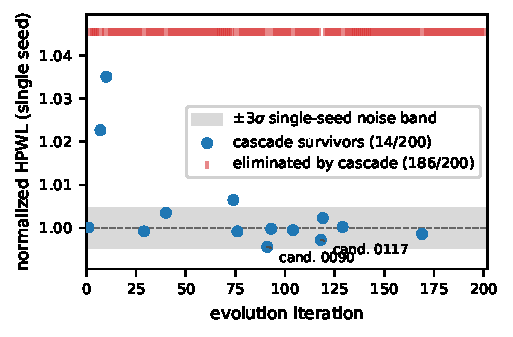
\includegraphics[width=\linewidth]{fig_evolution.pdf}
\caption{Single-seed scores of all 200 evolution candidates.
Survivor scores cluster inside the measured $\pm3\sigma$ noise band;
the cascade rejects 93\% of candidates cheaply (top ticks).}
\label{fig:evolution}
\end{figure}

\subsection{Multi-seed confirmation and the rank inversion}
Table~\ref{tab:rerank} and Figure~\ref{fig:rerank} give the paired
multi-seed outcome (5 seeds $\times$ 2 designs, 10 paired ratios per
program). The calibration row behaves: the seed program lands at
$1.00057\pm0.0074$, statistically indistinguishable from the default it
re-implements. The single-seed \emph{winner} (candidate 0090, single-seed
$0.99563$) regresses to exactly the baseline ($1.00014\pm0.0085$): its
$-0.44\%$ was seed luck. The single-seed \emph{runner-up} (candidate 0117,
single-seed $0.99716$) is the only real improvement:
$0.99685\pm0.0027$, i.e.\ $+0.315\%$ with a 95\% CI excluding zero
(${\approx}3.7\times$ SEM). Three additional programs included through a
record-keeping artifact (duplicate iteration indices in the result log
caused stale selections; they correspond to cascade-rejected programs)
serve as \emph{negative controls}: the protocol measures them $2.2$--$7.7\%$
worse with tight intervals, confirming sensitivity in both directions.

\begin{table}[t]
\centering
\caption{Paired multi-seed re-ranking (10 ratios per program; ratio
$<1$ improves on the default schedule at identical (design, seed)).}
\label{tab:rerank}
\footnotesize
\setlength{\tabcolsep}{3pt}
\begin{tabular}{lccc}
\toprule
Program & Single-seed & Paired mean $\pm$ std & Verdict \\
\midrule
cand.\ 0117 & 0.99716 & $0.99685 \pm 0.0027$ & \textbf{real, $+0.315\%$} \\
cand.\ 0090 & 0.99563 & $1.00014 \pm 0.0085$ & noise \\
seed (default) & 1.00010 & $1.00057 \pm 0.0074$ & calibration \checkmark \\
\midrule
neg.\ control A & --- & $1.02244 \pm 0.0059$ & worse (rejected) \\
neg.\ control B & --- & $1.06626 \pm 0.0046$ & worse (rejected) \\
neg.\ control C & --- & $1.07746 \pm 0.0123$ & worse (rejected) \\
\bottomrule
\end{tabular}
\end{table}

\begin{figure}[t]
\centering
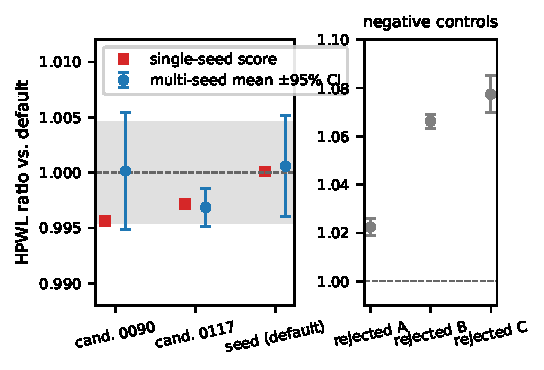
\includegraphics[width=\linewidth]{fig_rerank.pdf}
\caption{Single-seed score (squares) vs.\ paired multi-seed mean
$\pm$95\% CI (circles). The single-seed ranking inverts: the apparent
winner (0090) regresses to baseline; the runner-up (0117) is the real
improvement. Right: negative controls.}
\label{fig:rerank}
\end{figure}

\subsection{What the surviving schedule does}
The confirmed schedule (Figure~\ref{fig:schedules}) replaces the built-in
overflow-exponential heuristic with a blend of a cosine-warped geometric
decay and overflow-coupled terms, with a floor that prevents deep
annealing until \emph{both} schedule progress and density relaxation have
occurred. Qualitatively it anneals $\gamma$ later and more smoothly than
the default. The effect, however measurable, is small: $+0.315\%$ HPWL on
designs where the default schedule has been tuned for years.

\begin{figure}[t]
\centering
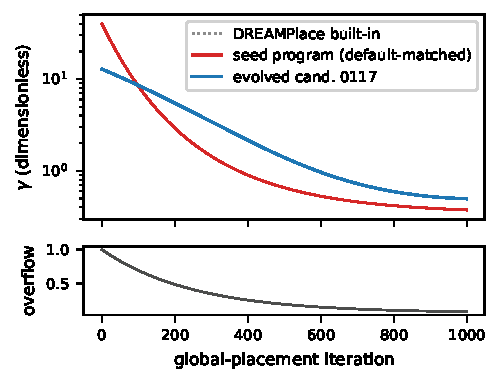
\includegraphics[width=\linewidth]{fig_schedules.pdf}
\caption{$\gamma$ trajectories under an illustrative overflow relaxation
(bottom): DREAMPlace's built-in heuristic, the default-matched seed
program, and the confirmed evolved schedule (cand.\ 0117).}
\label{fig:schedules}
\end{figure}

\subsection{An accidental third measurement}
After the campaign, visualization runs re-executed candidate 0117 and the
default on fresh seeds; the evolved schedule won by $+0.18\%$ and
$+0.27\%$ respectively---both within one standard error of the confirmed
$+0.315\%$ estimate, an incidental out-of-protocol replication.

\section{The $\lambda$ Campaign: Audit Beats Search}
\label{sec:lambda}

\subsection{An approximate seed and a $7\sigma$ gate flag}
DREAMPlace's density-weight update multiplies $\lambda$ by
$\mu = U\cdot\max(0.9999^{k},0.98)$ (with $U{=}1.05$) while HPWL improves
between evaluations, but shrinks $\mu$ through a feedback guard when HPWL
worsens. Our hook interface exposes (iteration, overflow, overflow
history, gradient norm, current $\lambda$) but not the HPWL deltas the
guard consumes, so a default-matched seed is not expressible; we seeded
with the improving-branch update applied \emph{unconditionally}. The
parity gate---which expects a default-matched seed to score
$1.0\pm0.01$---instead returned $0.9896$, a ${\sim}7\sigma$ deviation.
Under the protocol this is a stop condition: the discrepancy must be
explained before any search runs.

\subsection{Paired verification: the guard hurts}
\begin{figure}[t]
\centering
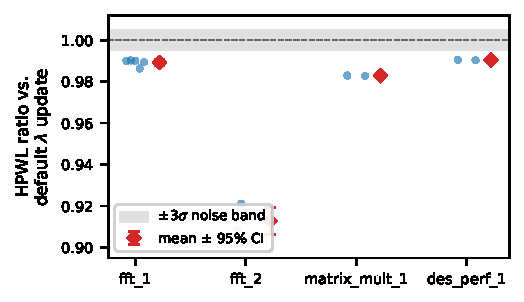
\includegraphics[width=\linewidth]{fig_lambda.pdf}
\caption{Guard-branch ablation: paired HPWL ratios vs.\ the default
$\lambda$ update at identical (design, seed), with matched final overflow.
All 14 pairs improve; the effect is design-heterogeneous (${\sim}1\%$ on
three designs, ${\sim}9\%$ on \texttt{fft\_2}).}
\label{fig:lambda}
\end{figure}
Paired re-evaluation (Fig.~\ref{fig:lambda}) attributes the deviation to
the guard itself: the unconditional ramp wins on \emph{every} pair ---
\texttt{fft\_1} $-1.0\%$ (5 seeds), \texttt{fft\_2} $-8.7\%$ (5 seeds),
\texttt{matrix\_mult\_1} $-1.7\%$ and \texttt{des\_perf\_1} $-1.0\%$
(2 seeds each) --- with final overflow matched to the default run in every
case (both flows reach the same density quality; the ablated schedule
reaches it at lower wirelength). Unlike the per-case-evolved components in
the literature, which lose an order of magnitude when generalized, this
single fixed change transfers across all four designs tested. We emphasize
the provenance: this is an \emph{ablation of a hand-tuned heuristic},
surfaced by a calibration gate, confirmed by the paired protocol ---
search played no role.

\subsection{Reward hacking and the density gate}
The initial $\lambda$ evolution run used the same HPWL-only fitness as the
$\gamma$ campaign. Within nine iterations a mutant scored an apparent
$-2.2\%$ ``improvement'' --- at final overflow $0.35$, five times the stop
criterion: the schedule simply suppressed the density ramp, leaving cells
clustered and wirelength artificially low. The $\gamma$ parameterization
cannot express this failure mode (smoothing does not control spreading);
the $\lambda$ parameterization can, and the search found it almost
immediately. We added a density gate (reject any candidate whose final
mean overflow exceeds $0.12$; defaults end at $0.07$--$0.085$) and
restarted. The contrast in search dynamics is stark: the ungated run
``improved'' repeatedly --- every gain a hack --- while the gated run
never improved at all.

\subsection{Gated evolution finds nothing}
Under the gate, 200 iterations of $\lambda$ evolution produced 150
candidates scored $-\infty$ (cascade or gate) and 49 survivors, all
$9$--$220\%$ worse than the seed; the unmodified seed remained the best
program. Combined with the $\gamma$ bound, the campaign-level conclusion
is symmetric and clean: \textbf{schedule search is noise-bounded in both
spaces; the only real win came from auditing the default's own adaptive
logic.}

\section{Discussion}

\textbf{Why the search headroom is small.} Three compounding causes. (i)~The
default schedule is already overflow-adaptive and extensively tuned; the
remaining gain from trajectory shaping of an optimizer that converges to
the same basin is intrinsically limited. (ii)~Standard-cell ISPD~2015
designs present smooth placement landscapes; the literature's large
evolved-component gains arise from \emph{macro} handling on macro-heavy
designs~\cite{yao2025evolution}, a lever these benchmarks barely expose.
(iii)~Effect sizes ($\leq0.3\%$) sit \emph{below} the single-seed noise
floor ($\sigma\approx0.15\%$, so single observations are dominated by
luck)---an evolutionary search cannot reliably climb a gradient its
fitness oracle cannot resolve, and our rank inversion shows the
consequence directly.

\textbf{The single-seed hazard is general.} Our campaign internally
reproduced, at small scale, the pattern documented in the RL-placement
reassessments~\cite{cheng2023assessment,markov2023false}: an uncalibrated
pipeline reports improvements that evaporate under controlled
re-evaluation. The protocol of Section~\ref{sec:protocol} is cheap
relative to any evolution campaign (here, ${\sim}70$ extra placements)
and catches both failure modes we encountered in practice---dead code
paths and noise-fitting---before they reach a results table.

\textbf{Search vs.\ audit.} The campaign's most useful contrast is
methodological. LLM search over schedule space, properly gated, recovered
at most $0.3\%$; a single ablation of a default heuristic, surfaced by a
calibration gate, recovered $1$--$9\%$ and generalized. Hand-tuned
adaptive heuristics inside mature placers have never been systematically
audited with variance-qualified methods, and our result suggests that
audit --- cheap, exhaustive, statistically grounded --- is currently a
better use of evaluation budget than search. The reward-hack episode adds
the operational corollary: any fitness a candidate can influence along an
unmeasured axis \emph{will} be exploited, and gates must be specified
with the objective, not patched in afterward.

\textbf{Consistency with concurrent work.} Yao et
al.~\cite{yao2025evolution} rank initialization $\gg$ optimizer $>$
preconditioner by both evolvability and gain, and report only
$0.03$--$0.59\%$ on their cleanest cases. Our schedule bound of
${\sim}0.3\%$ on standard-cell designs is quantitatively consistent with
their ordering, measured for a component class they did not study and
qualified with variance their study lacks.

\section{Conclusion}

We built a measurement-first harness for LLM-guided evolution of
DREAMPlace schedules and ran two complete, noise-calibrated campaigns on
ISPD~2015 standard-cell designs. The $\gamma$ campaign yields a bound:
one real improvement of $+0.315\%\pm0.09\%$ in 200 iterations, with the
single-seed ranking inverting under paired re-evaluation. The $\lambda$
campaign yields a discovery and a second bound: the default density-weight
update's HPWL-feedback guard actively hurts ($1$--$9\%$ at matched
density, $14/14$ paired seeds, four designs) --- found by the protocol's
parity gate, not by search --- while gated evolution atop the fix found
nothing further, after an ungated fitness was reward-hacked within nine
iterations. Together the campaigns quantify a previously unexamined
component class from both directions: schedule \emph{search} is
noise-bounded, schedule \emph{audit} is not. The enabling contribution is
the protocol --- noise-floor measurement, liveness and parity gates,
objective gates, and paired multi-seed confirmation with calibration
rows --- which caught a rank inversion, a non-parity seed worth $1$--$9\%$,
and a live reward hack, in a field where any of the three would normally
have shipped as a result.

\section*{Acknowledgments}
Experiments were carried out on an NVIDIA DGX Spark (GB10). The campaign's
laboratory notebook, all candidate programs, raw logs, and the evaluation
harness are available in the project repository.

\bibliographystyle{IEEEtran}
\bibliography{refs}

\end{document}
